\chapter{共享风险链路组分离路径算法研究}

\section{问题描述}
SRLG分离路径在它们之间没有任何共同的风险资源,也就是说,由于风险而导致的路径失败不会影响其他路径。图.\ref{fig:CompositeGraph}(b)显示两条SRLG分离路径对,表示为AP 和BP. 因为这两条路没有共同的风险资源,如果AP失败,BP仍然可以工作。本章主要讨论了两条不相交的路径保护路径,即可以描述如下。

\textbf{Min-Min SRLG分离路径问题}。给定一个图$G(V,E)$,每条链路$e_i\in \mathbb{E}$ 相关联一个权重权重$w_{e_i}$,一个源节点$s$和一个终结点$d$,找到一对$s$到$d$ 的SRLG分离路径对(表示为AP和BP),而且要求这两条分离路径中路径权重较小的那条路径权重最小化,形式如下:

\begin{equation}
\begin{array}{*{20}{c}}
   {\mathop {minimize}\limits_{AP,BP} } & {\min \left( {{w_{AP}},{w_{BP}}} \right)}  \\
   {subject\ to} & {{r_{AP}} \cap {r_{BP}}{\rm{ = }}\phi }  \\
   {} & {\mathbb{AP} \cap \mathbb{BP}{\rm{ = }}\phi }  \\
\end{array}
\label{eq:problem definition}
\end{equation}

即${w_{AP}}$ 和 ${w_{BP}}$是AP和BP的路径权重,$\mathbb{AP}$ 和 $\mathbb{BP}$分别是路径AP和BP上的链路集,${r_{AP}}$ 和 ${r_{BP}}$分别是影响路径AP和BP的SRLG集。


\begin{figure*}[tp]
  \centering
  % Requires \usepackage{graphicx}
  \includegraphics[width=7.2in]{figures/CompositeGraph}
  \caption{(a) A graph with five SRLGs: $\mathbb{R}_{r_1}=\{e_1,e_9\}$,$\mathbb{R}_{r_2}=\{e_2,e_3,e_{19}\}$,$\mathbb{R}_{r_3}=\{e_2,e_4,e_{11},e_{17}\}$,$\mathbb{R}_{r_4}=\{e_5,e_{13}\}$,$\mathbb{R}_{r_5}=\{e_{15},e_{18}\}$. (b)AP and BP in the graph. (c) The shortest weight path AP in the graph. $\mathbb{AP}=\{e_1,e_2,e_3,e_4,e_5,e_6,e_7,e_8\}$, $\mathbb{\mathbb{ER}}=\{e_9,e_{11},e_{17},e_{13},e_{19}\}$. (d)  Graph after deleting the links in $\mathbb{AP}$ and ${\mathbb{ER}}$. }
  \label{fig:CompositeGraph}
\end{figure*}

\section{原有算法概述}
共享风险链接组(SRLG)是一组链路共享相同的一个组件,该组件的故障会导致在这个组里所有链接的发生故障。就路径保护而言,尽管某些链路或者节点分离路径算法\cite{suurballe1984quick,bhandari1997optimal,li1990complexity,guo2003link,xu2004finding,beshir2011variants,guo2013finding,hu2003diverse} 已经提出来,SRLG分离路径 问题是比较棘手的,而且这些原有研究是限制在一定领域的。比如当每个SRLG只包含一条链路时,这个SRLG分离路由问题可以简化为链路分离路径问题,而通过节点分离方法(node split method)\cite{ford2015flows}节点分离路径问题可以转化为链路分离路径问题。因为SRLG组通常包括的链路超过一条并且网络中的链路通常可以属于多个SRLG组里,以至于求一对SRLG 分离路径问题比求一对链路或者节点分离路径问题要困难得多。

为了解决SRLG分离路径问题,一种可能的方法是0-1整数线性规划(ILP)\cite{hu2003diverse},通过分支限界法(branch-and-bound)来搜索来选择最优的主路径和备份路径。该方法时间复杂度高,不适用于大型网络。为了降低算法的复杂度,基于APF的启发式算法\cite{oki2002disjoint,li2002fiber,eppstein1998finding}能够求Min-Min SRLG分离路径问题的近似最优解。首先使用Dijkstra算法(或任何其他最短路径算法)求出主路径,求主路径时不考虑其相应的备用路径情况,在删除AP沿线的链路并且与AP共风险的节点和链路后,再利用最短路算法求的备用路径。

然而,使用APF启发式算法的有一个主要缺陷,一旦求得路径AP后也可能无法找到相对的SRLG分离路径BP,即使网络中确实存在一对分离路径。这就是所谓的“陷阱”问题,即使稠密网络中\cite{laborczi2001solving}这也是可能发生,在一个稀疏连接的网络中当然不能被忽略。陷阱有两种:不可避免的陷阱和可避免的陷阱。不可避免的陷阱是受拓扑约束的,任何算法都无法解决。如果网络不是2-边连通度的,则没有算法可以保证在拓扑中存在两个SRLG分离路径。另一方面,当两个节点之间存在SRLG分离路径对,但由于路由算法的缺陷而找不到时,就会出现一个可避免的陷阱。在本章中只考虑了可避免的陷阱。

对简单的APF算法的扩展,提出了KSP(K-最短路径)算法来处理节点/链路分离路径的陷阱问题。虽然它是处理陷阱问题最有效的算法之一,但它在大型网络中的性能受到影响,因为KSP 可能会涉及多路径搜索测试(K测试),直到它找到分离路径。当前候选的路径AP遇到陷阱问题后,仅根据路径长度选择下一个要测试的候选AP,而不考虑当前候选AP的那条链路(或那些链路)导致查找分离路径BP失败。因此,为了找到一对分离路径对,需要对大量的路径进行测试,这就引入了KSP算法中与K相关的时间复杂度。对于遇到陷阱问题的AP,我们应用从AP 路径导出的SRLG冲突链路集来指导将来的AP路径测试。这在很大程度上有助于减少寻找替代路径的时间复杂度。

其它SRLG分离路径算法\cite{rostami2012msdp,rostami2007cose,datta2008graph,xu2003new,todimala2004imsh},搜索最大SRLG分离路径对,并且路径间共享最小数目的公共链路。由于AP 和BP 可能具有相同的风险资源组,通过这种方法找到的解决方案是不可靠的。我们的算法目标是寻找完全SRLG分离路径。Xu\cite{xu2003trap}试图找到完全SRLG分离路径。但他的算法减少了问题的搜索空间,加快了路径搜索的速度。然而,它可能会以较大的代价返回路径,因为在削减后的空间可能会失去最优解。相反,为了大大加快搜索过程,我们利用SRLG冲突链接集将原问题划分为多个子问题,这些子问题可以并行执行。因此,我们的算法可以运行得更快,返回主路径成本非常低。

Datta\cite{datta2008graph}提出方法是将SRLG分离路径问题转化为链路分离路径问题,然后利用链路分离路径算法来解决。然而,只有特殊的SRLG模式(例如,星型)可以
将其转换为链路分离,这样就限制了该算法的广泛应用。当AP遇到陷阱问题时,CoSE\cite{rostami2007cose}算法试图找到一个SRLG集合,任何AP路径包含了这个SRLG集合里的所有SRLG,则必定找不到任何的与其对应的SRLG分离路径BP。CoSE 首先通过多轮搜索查找多个AP共享的SRLG,并且组成一个SRLG集合,然后根据SRLG集合来划分原始问题以搜索SRLG分离路径对。而不使用SRLG 中链路之间共享风险的特性,CoSE方法的这种穷尽搜索需要非常高的计算开销。



\section{整数规划形式化}
\section{时间复杂度}
\begin{theorem}
\label{le:lemma1}
    Min-Min SRLG-分离路径问题是 NP-complete.
\end{theorem}
\begin{proof}
根据\cite{bhatia2006finding},Min-Min链路分离路径问题是NP-complete的。Min-Min链路分离路径问题是Min-Min SRLG-分离路径问题的子问题。设
Min-Min SRLG分离路径问题的复杂性为C(A),则NP-complete的$\leq$C(A).

为了求Min-Min SRLG分离路径问题的时间复杂度,我们首先假设了一个问题B(问题B的复杂性表示为C(B)),当找到两条的SRLG分离路径并且路径较小的路径其权重小于或等于M(M是大于零整数数)。Min-mim SRLG分离路径问题A与问题B等价,我们知道M必须大于零并且小于$\sum\limits_{e_i\in \mathbb{E}}w_{e_i}$。例如,我们假设0≤M≤10和m=6是最优解,通过经典的二分法(binary search method)时间复杂度为O(log(N)),如图.\ref{fig:binarySearch}所示,通过二分法我们得到了两条分离的路径,较小的路径其权重为m,因此问题A与 问题B等价。
\begin{figure}[htp]
  \centering
  % Requires \usepackage{graphicx}
  \includegraphics[width=3.0in]{figures/binarySearch}
  \caption{Request optimal solution M through Binary search method }
  \label{fig:binarySearch}
\end{figure}
假设程序X在输入问题B时,如果问题B没有解,则程序Y立即停止,否则程序B继续执行并获得问题B的解,因此问题B可以归结为NP-硬停止问题。因此C(B)$\leq$NP-hard。

此外,给定任意两条路径,很容易在多项式时间内判别这两条路径是否为SRLG分离路径,较小的路径其权重小于或等于M,从而使得C(B)$\leq$NP-complete。当B的复杂度等于A时,我们有C(A)=C(B)$\leq$NP-complete。因此,A=NP-complete。
\end{proof}
\section{陷阱问题}
基于APF的启发式算法可能会陷入“陷阱”问题。也就是说,当一个AP被确定时,即使网络中确实存在一对分离路径对,它也可能无法找到SRLG分离的BP路径。图.\ref{fig:CompositeGraph}.(c),(d)说明了陷阱问题。虚线表示一个AP,其链路集为$\mathbb{AP}=\{e_1,e_2,e_3$ $,e_4,e_5,e_6,e_7,e_8\}$。在删除AP上的链路和与AP共享风险的链路后,图.\ref{fig:CompositeGraph}.(d) 所示的不存在从s到d的路径,因此找不到BP。

虽然KSP算法被认为是解决陷阱问题的有效算法,但它可能面临着效率低下的问题。在这个图.\ref{fig:KSPproblem}中,假设$e_1, e_2, e_3, e_4$的链路权重比其他链路大得多。此外,在$e_1, e_2, e_3, e_4$中,$e_1$ 和$e_2$的链接权重远小于$e_3$,$e_4$。然后,在KSP算法多次找从s到d的K短路时,总是包含$e_1,e_2$(虚线表示)。则最短AP 总会遇到陷阱问题,因为$e_1$和$e_4$ 具有相同的风险,因此无法找到BP。为了避免陷阱问题,必须将K设为一个大值,这给KSP带来了很高的时间复杂度。
\begin{figure}[htbp]
\centering
% Requires \usepackage{graphicx}
\includegraphics[width=2.8in]{figures/KSPproblem}
  \caption{An example to illustrate the inefficiency of KSP}
  \label{fig:KSPproblem}
\end{figure}


\section{分而治之的快速共享风险链路组分离路径算法}
当一个陷阱问题发生,并且对于给定的AP没有SRLG分离路径BP时,AP中可能存在一个子链路集,这样任何通过这个链路集里所有的这些“问题”链路的AP都不能找到一个SRLG分离BP。 我们称之为\textbf{SRLG冲突链路集}。与KSP不同,当最短AP遇到陷阱问题时,我们将通过两个主要步骤来解决这个问题。在图.\ref{fig:KSPproblem}的例子中,我们将首先找到图.\ref{fig:KSPproblem}中的SRLG冲突链路p集合,然后应用分而治之算法将原问题划分为两个子问题$\mathcal{P}(\emptyset,\{e_1\})$和 $\mathcal{P}(\{e_1\},\{e_2\})$。 这两个子问题可以在多核CPU平台上并行执行,快速得到SRLG分离路径对。
\subsection{分而治之}
在得到SRLG冲突链路集后,设计了一种分而治之的算法,将原Min-Min SRLG不相交路由问题划分为多个子问题,并行执行,加快求SRLG分离路径对的过程。

为了便于问题划分,我们首先用定义两个不相交的链接集和$\mathbb{I}$和$\mathbb{O}$,其中我被称$\mathbb{I}$为包含集集合,$\mathbb{O}$称为排除集集合。由$\mathcal{P}({\mathbb{I},\mathbb{O}})$表示的Min-Min SRLG-分离问题,用于寻找一对AP和BP,其中AP是所有可能的AP中最短的,其中路径$AP$必须经过$\mathbb{I}$集合里的所有链路和不经过$\mathbb{O}$集合里的所有链路

最初,让$\mathbb{I}=\emptyset$ 和 ${\mathbb{O}}=\emptyset$,原来的Min-Min SRLG分离路径对问题可以用$\mathcal{P}(\emptyset,\emptyset)$表示。给定SRLG冲突链路集$\mathbb{T}=\{{e_1},{e_2}, \cdots ,{e_{\left| \mathbb{T} \right|}}\}$,原问题$\mathcal{P}(\emptyset,\emptyset)$可按以下步骤划分。

\begin{enumerate}
  \item 首先,$\mathcal{P}(\emptyset,\emptyset)$能被划分成两个子问题$\mathcal{P}(\emptyset,\{e_1\})$ 和 $\mathcal{P}(\{e_1\},\emptyset)$。
  \item 类似,$\mathcal{P}(\emptyset,\{e_1\})$能被划分成两个子问题 $\mathcal{P}(\{e_1,e_2\},\emptyset)$ 和 $\mathcal{P}(\{e_1\},\{e_2\})$。
  \item 这个划分步骤持续直到步骤$|\mathbb{T}|$,问题$\mathcal{P}(\{e_1,e_2,\cdots ,{e_{\left| \mathbb{T} \right|-1}}\},\emptyset)$ 进一步的拆分成两个子问题$\mathcal{P}(\{e_1,e_2,\cdots ,{e_{\left| \mathbb{T} \right|-1}}, {e_{\left| \mathbb{T} \right|}}\},\emptyset)$ 和 $\mathcal{P}(\{e_1,e_2,\cdots ,{e_{\left| \mathbb{T} \right|-1}}\},{e_{\left| \mathbb{T} \right|}})$。注意到,子问题$\mathcal{P}(\{e_1,e_2,\cdots ,{e_{\left| \mathbb{T} \right|-1}}, {e_{\left| \mathbb{T} \right|}}\},\emptyset)$是无解的。
\end{enumerate}



除了子问题$\mathcal{P}(\{e_1,e_2,\cdots ,{e_{\left| \mathbb{T} \right|}}\},\emptyset)$外,我们将试图求其它每个子问题的最优解。然后选择最好的路径对(即最短路径对)。作为原问题$\mathcal{P}(\emptyset,\emptyset)$的最终(最优)解。如果这些子问题都没有解,则我们可以得出原问题没有任何解,因为我们子问题包括了所有的可能的分离路径对。

就时间复杂性而言,解决子问题所需的时间比原来的问题应该花费的更少。因为一条链路(来自集合$\mathbb{T}$)将在计算AP的路径时被去除,这也确保了不同的AP路径将被测试且是否存在一个SRLG分离BP路径。

当遇到陷阱问题时,我们的解决方案将划分原来的问题,并测试每个子问题以寻找到最终的解。在我们的分而治之方法中,子问题是由SRLG冲突链路集而得,而这个SRLG冲突链路集适是当AP路径遇到陷阱问题生成的。与现有的算法相比较,该算法在不考虑现有结果和问题的情况下,可以在很大程度上降低算法的计算量。对于图.\ref{fig:DividedConquer}中的例子所示,SRLG冲突链接集是$\mathbb{T}=\{e_2,e_5,e_6\}$。拆分过程过程如图.\ref{fig:DividedConquer}所示。根据SRLG冲突链路集,我们应该测试总共3个子问题${{\mathcal{P}}(\{ e_2,e_5\} ,\{ e_6\} )}$, ${{\mathcal{P}}(\{ e_2\} ,\{ e_5\} )}$ 和 ${{\mathcal{P}}(\emptyset ,\{ e_2\} )}$,其中选择AP路径权重最低的最优子问题作为原问题$\mathcal{P}(\emptyset,\emptyset)$最终的(最优)解。

注意,我们不需要解决子问题${{\mathcal{P}}(\{ e_2,e_5\}, \emptyset)}$ 和 ${{\mathcal{P}}(\{ e_2\},\emptyset )}$,因为它们的解已经包含在其它的子问题中。第一个解空间由两个子问题${{\mathcal P}(\{ e_2,e_5,e_6\} ,\emptyset )}$ 和 ${{\mathcal P}(\{ e_2,e_5\} ,\{ e_6\} )}$组成。由于SRLG冲突链接集为$\mathbb{T}=\{e_2,e_5,e_6\}$,显然,子问题${{\mathcal P}(\{ e_2,e_5,e_6\} ,\emptyset )}$是没有解的。因此,${{\mathcal P}(\{ e_2,e_5\} ,\{ e_6\} )}$的解空间等于${{\mathcal{P}}(\{ e_2, e_5\}, \emptyset)}$的解空间。同样,${{\mathcal{P}}(\{ e_2\},\emptyset )}$的解空间包括${{\mathcal{P}}(\{ e_2\} \{ e_5\}, \emptyset)}$  和 ${{\mathcal{P}}(\{ e_2\} ,\{ e_5\} )}$的解空间。
\begin{figure}[htbp]
\small{
\begin{equation*}
{\mathcal P}(\emptyset ,\emptyset )\left\{ {\begin{array}{*{20}{l}}
{{\mathcal P}(\{ e_2\} ,\emptyset )\left\{ {\begin{array}{*{20}{l}}
{{\mathcal P}(\{ e_2,e_5\} ,\emptyset )\left\{ {\begin{array}{*{20}{l}}
{{\mathcal P}(\{ e_2,e_5,e_6\} ,\emptyset )}\\
{\boxed{{\mathcal P}(\{ e_2,e_5\} ,\{ e_6\} )}}
\end{array}} \right.}\\
{\boxed{{\mathcal P}(\{ e_2\} ,\{ e_5\} )}}
\end{array}} \right.}\\
{\boxed{{\mathcal P}(\emptyset ,\{ e_2\} )}}
\end{array}} \right.
\end{equation*}
}
\caption{Example to illustrate divide-and-conquer solution}
\label{fig:DividedConquer}
\end{figure}




\subsection{SRLG冲突链路集合}
在本节中,我将描述了如何找到一个SRLG冲突链路集合,当在网络$G$中给定一个AP路径并且没有SRLG分离的BP路径。
\subsubsection{通过新奇的边容量设置准则构造一个新的图$G^*$}
如\ref{subsubsec:maxFlow}节介绍的,如果在图G中去除所有在边割集$\mathbb{\mathbb{L}}_{\Phi}$的所有边,则$|f| = 0$。也就是说,不存在任何流能从$s$到$d$。在本文中,我们试图基于割集的概念找到SRLG冲突链路集合。如果AP从s到d流通,经过的链路与割集$\mathbb{\mathbb{L}}_{\Phi}$共享风险,则找不到任何与其对应的SRLG分离路径BP,因为没有一条在割集中的链路可以被BP选择。

基于割集上基础上为了找到SRLG 冲突链路集,我们构造了一个新的图$G^*$ ,如下所示.
\begin{enumerate}
  \item $G^*$与$G$的节点和链路结构一样
  \item 跟每条链路$e_i$相关的链路权重$w_{e_i}$是跟其相对应图$G$中边的权重一样的。
  \item 我们使用以下准则设置每条边$e_i \in \mathbb{E}$相关的容量$c_{e_i}$
\end{enumerate}
 \begin{equation}
c_{e_i} = \left\{ {\begin{array}{*{20}{c}}
   1 & {e_i{\rm{ }} \in {\rm{ \mathbb{AP}}}}  \\
   {\left| \mathbb{AP} \right|+1} & {e_i{\rm{ }} \in {\rm{ \mathbb{E}}}{{\rm{\mathbb{R}}}}}  \\
   {\left| {{\rm\mathbb{AP}}} \right| + \left( {\left| {{\rm\mathbb{AP}}} \right| + 1} \right)\times \left| {{\rm{\mathbb{E}}}{{\rm{\mathbb{R}}}}} \right| + 1} & {otherwise}  \\
\end{array}} \right.
\label{eq:capacity principle}
\end{equation}
$\mathbb{AP}$指在图$G$中较小权重路径$AP$上所有链路的集合,和$\mathbb{\mathbb{ER}}$指不属于路径$AP$上的边但是与路径$AP$上的边共享风险的链路集合。

在图.\ref{fig:CompositeGraph}(c)所示,路径$AP$的边集合$\mathbb{AP}=\{e_1,e_2,e_3,e_4$
$,e_5,e_6,e_7,e_8\}$, $\mathbb{\mathbb{ER}}=\{e_9,e_{11},e_{17},e_{13},e_{19}\}$。$|\mathbb{AP}|=8$, $|\mathbb{\mathbb{ER}}|=5$, $|\mathbb{AP}|+1=9$ 和 ${\left| {{\rm{\mathbb{AP}}}} \right| + \left( {\left| {{\rm{\mathbb{AP}}}} \right| + 1} \right)\times \left| {{\rm{\mathbb{E}}}{{\rm{\mathbb{R}}}}} \right| + 1}=54$. 我们产生一个新图$G^*$如图.\ref{fig:FlowStarGraph}所示, 在图$G^*$中边的容量是根据公式.(\ref{eq:capacity principle})所设置.

\begin{figure}[tp]
  \centering
  % Requires \usepackage{graphicx}
  \includegraphics[width=3.6in]{figures/FlowStarGraph}
  \caption{New Graph $G^*$}\label{fig:FlowStarGraph}
\end{figure}

\subsubsection{新图$G^*$中最小割集的性质}
最大流最小割定理指出,在网络中,从源节点$s$到目的节点$d$最大流值等于最小边割集的总容量,即最小的链路总容量,如果删除最小边割集上的边,将断开目的节点$d$与源节点$s$的连通。 我们的算法基于图的最小割集的链路集来求得最小SRLG 冲突链路集。

我们将首先展示我们重建新图$G^*$的一些优良特性为求得最小SRLG冲突链路集。

\begin{lemma}
\label{le:lemma1}
    在图$G^*$任何从$s$到$d$的路径必须经过一条边在边集合 $\mathbb{AP}$ 或者 $\mathbb{\mathbb{ER}}$中。
    %note:draw a picture to describe the proof
\end{lemma}
\begin{proof}
我们用矛盾的方法证明这条引理。假设对于某条路径AP,有另一条路径从$s$到$d$在图$G^*$中不与AP共享风险,即这条路径不通过$\mathbb{AP}$ 或者 $\mathbb{\mathbb{ER}}$的任何一条链路。我们可以很容易得出这样的结论,这条路径是与路径AP对应的SRLG分离路径BP。这与AP没有对应的SRLG分离路径的说法相矛盾。
\end{proof}

\begin{lemma}
\label{le:lemma2}
    图$G^*$的任何一条最大流的流值是最多为$|\mathbb{AP}|+(|\mathbb{AP}|+1)\times|\mathbb{\mathbb{ER}}|$。
\end{lemma}
\begin{proof}
假设$G^*$的最大流f为$|f|=k$。在$G^*$中,f可以被划分为k个从s到d的1单元流。根据引理.\ref{le:lemma1},这些1单位流中的每一个都必须通过通过$\mathbb{AP}$ 或者 $\mathbb{\mathbb{ER}}$的至少一个链路。请注意,$\mathbb{AP}$ 或者 $\mathbb{\mathbb{ER}}$ 中链路的容量分别为1或者$|\mathbb{AP}|$+1。根据$\mathbb{AP}$ 和 $\mathbb{\mathbb{ER}}$中链路的容量设置,因为$\mathbb{AP}$中的链路只能承载1单位流量,而在ER中,一条链路在$\mathbb{ER}$中能最多承载$|\mathbb{AP}|$+1单位流量.因此,最多只能有$|\mathbb{AP}|+ (|\mathbb{AP}|+1)\times|\mathbb{\mathbb{ER}}|$个从s到d的单位流量。
\end{proof}

\begin{lemma}
\label{le:lemma3}
    图$G^*$的最小割$\Phi$的边割集$\mathbb{L}_{\Phi}$所有链路都在$\mathbb{AP}$ 或者$\mathbb{\mathbb{ER}}$中。
\end{lemma}

\begin{proof}
根据最大流最小切定理,$c(\Phi)$表示的最小切割$\Phi$的的容量,其应该等于最大流量值,根据引理 \ref{le:lemma2}最大流量最多为$|\mathbb{AP}|+ |\mathbb{ER}|\times (|\mathbb{AP}|+1)$。 根据容量设定原则如公式\ref{eq:capacity principle}所示,一条链路既不在$\mathbb{AP}$ 也不在 $\mathbb{ER}$ ($e_i \notin \mathbb{AP}$ 和 $e_i \notin \mathbb{ER}$), 这条链路的容量为 $c_{e_i} = \left| {{\rm\mathbb{AP}}} \right| + \left( {\left| {{\rm\mathbb{AP}}} \right| + 1} \right)\times \left| {{\rm{\mathbb{E}}}{{\rm{\mathbb{R}}}}} \right| + 1$, 这条链路是大于$|\mathbb{AP}|+(|\mathbb{AP}|+1)\times |\mathbb{ER}|$. 因此,这条链路不可能在$\mathbb{L}_{\Phi}$中. 因此,割集$\mathbb{L}_{\Phi}$中的所有链路都必须属于边集合$\mathbb{AP}$ 或者 $\mathbb{ER}$。
\end{proof}


\begin{theorem}
    如果在图$G$中一个单元流阻塞了全部边割集$\mathbb{L}_{\Phi}$的所有边,则在原图中不会存在任何流经过这个图的割。
\label{th:block flow}
\end{theorem}


\begin{proof}
    如果在图$G$中一个单元流阻塞了全部边割集$\mathbb{L}_{\Phi}$的所有边,则在原图中没有流能使用边割集$\mathbb{L}_{\Phi}$ 里的边和没有任何流能经过这个图的割。
\end{proof}
定理\ref{th:block flow}提供了找到SRLG冲突链路集的可能性。即当AP路径遇到陷阱问题时,我们找到$\mathbb{AP}$路径边集的子集能够阻塞国有在边割集$\mathbb{L}_{\Phi}$的所有边,和这个子集即SRLG冲突链路集。当一条路径包含SRLG冲突链路集里的所有边,则没有任何流能经过割集$\Phi$,因此没有与其对应的SRLG分离路径BP。

\subsubsection{SRLG冲突链路集的集合覆盖问题}
虽然AP路径上的所有链接一起构成了SRLG冲突链接集,我们感兴趣的是一个集,它的数量很少链接,作为SRLG冲突链接集的大小确定分区的子问题数。调至V-B节。

根据定理2,最小SRLG冲突链接集查找问题可以描述为:查找AP上的最小链接子集,这些链接可以阻塞割集LΦ

对于任何链接ei,让sredenote链接集分担风险。和EI。显然,Sreicover本身和所有的链接包括EI在内的SRLG。例如,在图8中,e2是在两个SRLG中SRLGs $\mathbb{R}_{r_2}=\{e_2,e_3,e_{19}\}$, $\mathbb{R}_{r_3}=\{e_2,e_4,e_{11},e_{17}\}$, therefore, $\mathbb{SR}_{e_2}=\{e_2,e_3,e_{19},e_4,e_{11},e_{17}\}$.


For any link $e_i$, let $\mathbb{SR}_{e_i}$ denote the link set that shares risks with $e_i$. Obviously, $\mathbb{SR}_{e_i}$ covers $e_i$ itself and all the links in the SRLG that includes $e_i$. For example in Fig.\ref{fig:MinCutStarGraph}, as $e_2$ is in two SRLGs $\mathbb{R}_{r_2}=\{e_2,e_3,e_{19}\}$, $\mathbb{R}_{r_3}=\{e_2,e_4,e_{11},e_{17}\}$, therefore, $\mathbb{SR}_{e_2}=\{e_2,e_3,e_{19},e_4,e_{11},e_{17}\}$.

For each link $e_i$ on AP, we define its cut-block-link set as ${\mathbb{B}_{{e_i}}} = \mathbb{SR}_{{e_i}} \cap \mathbb{L}_{\Phi}$, which is the sub-set of \textbf{cut-set} $\mathbb{L}_{\Phi}$ that can be blocked by $e_i$.

因此,最小SRLG冲突链路集查找问题可以表述为集覆盖问题:给定AP(AP的路径链接集)、剪切集LΦ和集合的剪切块链接集。

Therefore, the minimum SRLG Conflicting Link Set finding problem can be formulated as a Set Cover Problem: given $\mathbb{AP}$ (the link set of path links of $AP$), the \textbf{cut-set} $\mathbb{L}_{\Phi}$,  and a collection of the cut-block-link sets ${\mathbb{B}_{{e_1}}},{\mathbb{B}_{{e_2}}}, \cdots ,{\mathbb{B}_{{e_{|\mathbb{AP}|}}}}$, we want to find the fewest sets whose union is $\mathbb{L}_{\Phi}$, that is, the smallest $\mathbb{T} \subseteq \{e_i| e_i\in \mathbb{AP}\}$ such that ${ \cup_{e_i \in \mathbb{T}}}{\mathbb{B}_{e_i}} = \mathbb{L}_{\Phi}$.


\begin{figure*}[tp]
  \centering
  % Requires \usepackage{graphicx}
  \includegraphics[width=3.8in]{figures/MinCutStarGraph}
  \caption{Min cut of the network graph, $\mathbb{SR}_{e_1}=\{e_1, e_9\},\mathbb{SR}_{e_2}=\{e_2,e_3,e_4, e_{11},e_{17},e_{19}\},\mathbb{SR}_{e_3}=\{e_2,e_3, e_{19}\},\mathbb{SR}_{e_4}=\{e_2,e_4, e_{11},e_{17}\},\mathbb{SR}_{e_5}=\{e_5, e_{13}\},\mathbb{SR}_{e_6}=\{e_6\},\mathbb{SR}_{e_7}=\{e_7\} $ and $\mathbb{SR}_{e_8}=\{e_8\}$. $\mathbb{L}_{\Phi}=\{e_{11},e_{13},e_{19},e_{6}\}$. $\mathbb{B}_{e_1}=\emptyset,\mathbb{B}_{e_2}=\{e_{11},e_{19}\},\mathbb{B}_{e_3}=\{e_{19}\},\mathbb{B}_{e_4}=\{e_{11}\},\mathbb{B}_{e_5}=\{e_{13}\},\mathbb{B}_{e_6}=\{e_6\}$,$\mathbb{B}_{e_7}=\emptyset$ and $\mathbb{B}_{e_8}=\emptyset$.}\label{fig:MinCutStarGraph}
  \label{fig:MinCutStarGraph}
\end{figure*}

The Set Cover Problem is usually an NP-hard problem with its complexity depending on the size of the elements (denoted by $n$). In our minimum SRLG Conflicting Link Set finding problem, $n=|\mathbb{L}_{\Phi}|$, that is, the edge number of cut set $\mathbb{L}_{\Phi}$. As this paper's focus is not to improve the solution of the set cover problem, we apply the algorithm proposed in \cite{chvatal1979greedy} with the complexity $O(log(|\mathbb{L}_{\Phi}|))$  to find the minimum SRLG Conflicting Link Set. Usually, even for a large scale network, the  AP with the shortest path does not have a large number of $n=|\mathbb{L}_{\Phi}|$. Therefore, the cost to calculate the minimum SRLG Conflicting Link Set through the set cover is not large.

To illustrate how to find the minimum SRLG Conflicting Link Set, we show an example in Fig.\ref{fig:MinCutStarGraph}. For the min-cut $\Phi(\mathbb{S},\mathbb{D})$, $\mathbb{S}=\{s, 1, 2, 3, 4, 5, 9\}$ and $\mathbb{D}=\{d, 6, 7, 8\}$, the \textbf{cut-set} is $\mathbb{L}_{\Phi}=\{e_{11},e_{13},e_{19},e_{6}\}$. For links in $\mathbb{AP}$,  cut-block-link sets are: $\mathbb{B}_{e_1}=\emptyset$, $\mathbb{B}_{e_2}=\{e_{11},e_{19}\}$, $\mathbb{B}_{e_3}=\{e_{19}\}$, $\mathbb{B}_{e_4}=\{e_{11}\}$, $\mathbb{B}_{e_5}=\{e_{13}\}$, $\mathbb{B}_{e_6}=\{e_6\}$, $\mathbb{B}_{e_7}=\emptyset$ and $\mathbb{B}_{e_8}=\emptyset$. To cover $\mathbb{L}_{\Phi}$, the fewest cut-block-link sets are $\{\mathbb{B}_{e_2}$, $\mathbb{B}_{e_5}$, $\mathbb{B}_{e_6}\}$. Therefore, the minimum SRLG Conflicting Link Set is $\mathbb{T}=\{e_2, e_5, e_6 \}$.

In the example of Fig.\ref{fig:MinCutStarGraph}, although $|\mathbb{L}_{\Phi}|=4$, the size of  the minimum SRLG Conflicting Link Set $|\mathbb{T}|=|\{e_2, e_5, e_6 \}|=3$ is even smaller than $|\mathbb{L}_{\Phi}|=4$. This is because $e_2$ belongs to   SRLGs $\mathbb{R}_{r_2}$ and $\mathbb{R}_{r_3}$, and can block two links in $e_{11}$ and  $e_{19}$ in the \textbf{cut-set} $\mathbb{L}_{\Phi}$.

According to the graph style of SRLG, there are two categories \cite{datta2008graph}:  star-style and none star-style. For star-style SRLG, all the links start from the same node or ends at the same node. For example, in Fig.\ref{fig:MinCutStarGraph}, $e_1$ and $e_9$ start from the  the same node $s$, $\mathbb{R}_{r_1}$ is a star-style SRLG.  For none star-style SRLG, not all links in the SRLG starting from the same node or ending at the same node. In Fig.\ref{fig:MinCutStarGraph}, $\mathbb{R}_{r_2}$, $\mathbb{R}_{r_3}$, $\mathbb{R}_{r_4}$ and $\mathbb{R}_{r_5}$ are none star-style SRLGs.
Moreover, even though Fig.\ref{fig:MinCutStarGraph} includes both  star-style SRLG  and none star-style SRLG,  our  algorithm works efficiently and effectively to find the conflicting set through the solving of the set cover problem.

Therefore, different from some existing studies \cite{datta2008graph} which can only handle a single SRLG style or a simple scenario such as  one link belonging to only one SRLG, our algorithm works effectively in a more  general scenario that a link can belong to one or multiple SRLGs with more diverse SRLG styles.



\subsection{算法步骤}
在本节中,我们首先介绍我们的完整解决方案,然后分析其复杂性。

算法1显示完全min-min srg不相交。路由算法算法中的输入参数包括网络图(G)、源(S)、目标(D)应将包含链接集包括在AP(I)中,以及排除链路集不应包含在AP(O)中。算法的输出是SRLG不相交路径对。(美联社,BP)。

Algorithm \ref{alg:min-min} shows the complete min-min SRLG disjoint routing Algorithm. The input parameter in the algorithm includes  the network graph ($G$), the source ($s$), the destination  ($d$), the inclusion link set should be included in AP ($\mathbb{I}$), and the exclusion link set should not be included in AP ($\mathbb{O}$). The output of the algorithm is the SRLG disjoint path pair $(AP,BP)$.


寻找SRLG不相交的路径,最小的首先搜索网络中的权重ap在步骤2中找到AP(G,s,d,i,O),其中i=φ,O=φ,然后通过查找srlg不相交的bp对bp进行搜索。(g,s,d,AP)第4步。特别是,AP路径可以是通过Dijkstra算法发现的。为了计算BP,发现SRLG不相交BP(G,s,d,AP)包括两个步骤。首先,对于AP上的所有链接,删除共享这些链接的共同风险。第二,Dijkstra算法再次运行网络的其余链接来计算。从s到d的第二条最短路径BP。


To look for the SRLG disjoint paths, the smallest weight AP in the network is searched  first through FIND\_AP$(G,s,d, \mathbb{I},\mathbb{O})$ in step \ref{alg:findap} with $\mathbb{I}=\phi,\mathbb{O}=\phi$, and then BP is searched through  FIND\_SRLG\_Disjoint\_BP
$(G,s,d,AP)$ in step \ref{alg:findsrlgdisjointbp}. Specially, the AP path can be found through the Dijkstra algorithm. To calculate BP, FIND\_SRLG\_Disjoint\_BP
$(G,s,d,AP)$ includes two steps. First, for all the links on the AP, remove the links that share a common risk with these links. Second, the Dijkstra's algorithm runs over the remaining links of the network again to compute the second shortest path BP from $s$ to $d$.


如果我们能找到一个srg不相交的bp,那么Min-Min srlg解决了不相交的路由问题,找到了路径对。返回,如步骤6所示。否则,陷阱问题发生了。要处理陷阱问题,步骤8首先找到SRLG冲突链接集T,步骤10进一步划分原Min-Min SRLG不相交路由问题到T子-基于冲突集的问题T.所有的子问题都可以并行执行。步骤11利用集合F存储满足APi 6=φ和BPI 6=φ的可行解。在F中的所有可行解中,具有选择最低的AP路径权重作为最优解。对于原Min-Min SRLG不相交路由问题


If we can find a SRLG-Disjoint BP, the Min-Min SRLG disjoint routing problem is solved and  the path pair found is returned as shown in step \ref{alg:returnpathpair}. Otherwise, a trap problem happens. To handle the trap problem, step  \ref{alg:findsrlgconflictinglinkset} first finds the SRLG Conflicting Link Set $\mathbb{T}$, step \ref{alg:dividedandconquer} further divides the original  Min-Min SRLG disjoint routing problem into $\left| \mathbb{T} \right|$ sub-problems based on the conflict set $\mathbb{T}$. All the sub-problems can be executed in parallel. Step \ref{alg:findfeasible} utilizes the set $\mathbb{F}$ to store the feasible solutions  satisfying that  both $A{P_i} \ne \phi$ and $B{P_i} \ne \phi$. Among all the feasible solutions in the $\mathbb{F}$, the path pair with the lowest AP path weight will be selected as the optimal solution for the original Min-Min SRLG disjoint routing problem.


我们以图3中的图表为例来说明算法1.根据步骤2,我们的算法首先搜索对于路径AP={e1,e2,e3,e4,e5,e6,e7,e8}具有最小的通过Dijkstra算法加权,路径显示为图3(C)中的虚线。删除AP 上的链接后此外,与AP有共同风险的链接,我们有图3(D)中的图,这是一个不连通图,找不到BP。然而,如图3(B)所示,拓扑中存在SRLG-不相交路径对.因此,陷阱问题就会发生。在找到SRLG 冲突链接之后设置{e2,e5,e6}在步骤8中,我们对将原问题P(∅,∅)分为三个子问题,P(∅,{e2}),P({e2},{e5})和P({e2,e5},{e6})第10步。并行执行这些子问题之后,返回具有最小AP权重的路径对。


We take the graph in Fig.\ref{fig:CompositeGraph} as an example to illustrate  our Algorithm \ref{alg:min-min}.
According to step $\ref{alg:findap}$, our  algorithm first searches for a path  $\mathbb{AP}=\{e_1,e_2,e_3,e_4,e_5,e_6,e_7,e_8\}$ with the smallest weight through the dijkstra algorithm, with the path shown as the dotted line in Fig.\ref{fig:CompositeGraph}(c). After removing the links on AP and also the links that share the common risks with AP, we have the graph in Fig.\ref{fig:CompositeGraph}(d), which is a disconnected graph and no BP can be found. %\note{You gave the exact example earlier. Dear sister, from the previous comments, we find we need a example to illustrate the how our algorithm runs}
However, as shown in Fig.\ref{fig:CompositeGraph}(b), there exists a SRLG-disjoint path pair in the topology. Therefore, a trap problem happens. After finding the SRLG conflict link set $\{e_2,e_5,e_6\}$ in step $\ref{alg:findsrlgconflictinglinkset}$, we apply divide and conquer to divide the original problem ${\mathcal P}(\emptyset ,\emptyset )$  into three sub-problems, ${\mathcal P}(\emptyset ,\{e_2\} )$, ${\mathcal P}(\{e_2\} ,\{e_5\} )$ and ${\mathcal P}(\{e_2,e_5\} ,\{e_6\} )$ according to step $\ref{alg:dividedandconquer}$. After executing these sub-problems in parallel, the path pair with the minimum AP weight is returned.

 %For example, subproblem ${\mathcal P}(\{e_2\} ,\{e_5\} )$ obtain a AP ($e_1,e_2,e_3,e_{11},e_{12},e_8$) whose corresponding BP ($e_15,e_18,e_3,e_6,e_7,e_{14}$). compare the AP's weight of ${\mathcal P}(\{e_2\} ,\{e_5\} )$  with other parellel subproblems in order to obtain optimal solution. subproblem ${\mathcal P}(\emptyset ,\{e_2\} )$ obtain a AP ($e_9,e_3,e_4,e_5,e_6,e_7,e_8$) which result finding no BP, so continue divide and conquer subproblem ${\mathcal P}(\emptyset ,\{e_2\} )$ as like Alg.\ref{alg:min-min} step 8.}

\begin{algorithm}
\small{
\caption{Min-Min}
\begin{algorithmic}[1]
\label{alg:min-min}
%\caption{Main process of Algorithm}
\REQUIRE
$G$: the network graph\\
$s$: the source node\\
$d$: the destination node \\
$\mathbb{I}$:   the inclusion link set should be included in AP\\
$\mathbb{O}$: the exclusion link set should not be included in AP\\
\ENSURE
AP: the active path\\
BP: the backup path
\STATE $AP=\emptyset$, $BP=\emptyset, \mathbb{I}=\emptyset, \mathbb{O}=\emptyset$
\STATE $AP\leftarrow$ FIND$\_$AP$(G,s,d,\mathbb{I},\mathbb{O})$\label{alg:findap}
\IF{$AP\neq\emptyset$}
    \RETURN $BP\leftarrow$ FIND\_SRLG\_Disjoint\_BP$(G,s,d,AP)$\label{alg:findsrlgdisjointbp}
    \IF{$BP\neq\emptyset$}
        \RETURN {path pair $(AP,BP)$}\label{alg:returnpathpair}
    \ELSE
        \STATE find SRLG Conflicting Link Set $\mathbb{T}$\label{alg:findsrlgconflictinglinkset}
        \STATE $\mathbb{T}\leftarrow \mathbb{T}-(\mathbb{I}\cup\mathbb{O})$
        %\IF{$\mathbb{T}\neq \emptyset$}
        \STATE {divide and conquer for execution in parallel\\
        \tiny{
        $\!\!\!\!\!\!\!\!\!\!\!\!\!\!\!\!\!\!\!\left\{ \begin{array}{l}
 \left( {A{P_1},B{P_1}} \right)={{Min-Min}}\left( {G,s,d,\mathbb{I} ,\mathbb{O}\cup\{ {t_1}\} } \right), \\
 \left( {A{P_2},B{P_2}} \right)={{Min-Min}}\left( {G,s,d,\mathbb{I}\cup\{ {t_1}\} ,\mathbb{O}\cup\{ {t_2}\} } \right), \\
 \left( {A{P_3},B{P_3}} \right)={{Min-Min}}\left( {G,s,d,\mathbb{I}\cup\{ {t_1},{t_2}\} ,\mathbb{O}\cup\{ {t_3}\} } \right), \\
  \cdots  \\
 \left( {A{P_{\left| \mathbb{T} \right|}},B{P_{\left| \mathbb{T} \right|}}} \right) = {{Min-Min}}\left( {G,s,d,\mathbb{I}\cup \{ {t_1},{t_2}, \cdots ,{t_{\left| \mathbb{T} \right| - 1}}\} ,\mathbb{O}\cup\{ {t_{\left| \mathbb{T} \right|}}\} } \right) \\
 \end{array} \right.$
 }
        }\label{alg:dividedandconquer}
        \STATE{  {$\!\!\!\!\!\!\!\!\!\!\!F\leftarrow$ FIND\_FEASIBLE$(( {A{P_1},B{P_1}} )),\cdots,( {A{P_{|\mathbb{T} |}},B{P_{| \mathbb{T} |}}} )$}}\label{alg:findfeasible}
        %\ENDIF
         \IF{$F\neq{\emptyset,\emptyset}$}
         \RETURN{path pair $(AP,BP)$ satisfying that $AP = \mathop {\arg \min }\limits_{AP} \left\{ F \right\}$}
        \ENDIF

    \ENDIF
\ENDIF
\end{algorithmic}
}
\end{algorithm}


\subsection{时间复杂度}
若要在AP遇到时查找SRLG不相交路径对,请执行以下操作一个陷阱问题,我们的算法首先计算SRLG。冲突链接集,然后通过把它划分成T个子问题。如节所述切集LΦ的边数通常不大,因此,本文寻找SRLG冲突链路集。不会带来太多的成本。因此,我们关注的是路径查找过程的计算开销。

一般来说,对于一个有E连接和V节点的网络,求最小权路径的复杂性是(E)。(V)log(V)。为了解决陷阱问题,我们的路径发现问题与最初的最小重量有点不同。路径查找问题。我们引入了路径的一些约束条件。例如,查找AP路径必须通过链接集。或者不能通过一组。由于这些链接集通常并不大,这些约束在成本计算上几乎没有差别。如不同的子问题有不同的链接集,因此不同。复杂性,为了使描述简单明了,我们仍然使用(EV)log(V)作为一次路径搜索。作为我们算法将原问题分成T个子问题,算法复杂度为T(EV)log(V)。

对于复杂性的比较,我们也展示了复杂性。的路径发现过程,在Cose[28]和KSP[23]。

Cose试图找到一个冲突的SRLG集,而不是一个冲突链接集,就像我们所做的。虽然他们在寻找冲突的SRLG集是穷尽的,成本很高。本文主要研究路径发现过程的成本分析。在比较中不要考虑到这一成本。由于我们的SRLG冲突链接集来自min-裁剪和集合覆盖问题,T是最小的。SRLG冲突链接集的大小。因此,在Cose中冲突的SRLG集至少是T,并且我们表示SRLG集合为SRLG 1,SRLG 2,···,SRLG T?由于每个srlg路径包含多个链接,因此子问题。分区应该比我们的要大得多。在SRLG问题分区的过程包括SRLG链接,包含或排除SRLG链接在AP中会产生SRLG子问题。所以一个S-RLG集?SRLG 1,SRLG 2,···,SRLG T?将介绍T型qi=1个SRLGi子问题,作为链接组合(从SRLG提取每个链接以将其从(陷阱)对应一个子问题。因此,复杂性柯斯t qI=1 SRLGi(E V)log(V),即比我们的大得多。

对于KSP[23],路径查找复杂度为K((E))。(V)log(V),其中K是第一个K的最短数。在发现SRLG不相交之前应该测试的路径BP。然而,由于KSP没有从前面的路径搜索过程,在最坏的情况下,是ksp。应该尝试从源到目标的所有路径。因此,最糟糕的K值是2E,这会带来很大的影响。计算量大。

因此,相对于成本[ 28 ]和KSP [ 23 ],我们
算法利用最小割理论来减少
这样搜索的路径具有最小的计算成本。在
第viii-b3,我们将进一步提供广泛的模拟
证明我们的算法可以达到很高的效果。
计算速度找到SRLG不相交的路径使用
拓扑跟踪数据。

To find a SRLG disjoint path pair when an AP encounters a trap problem, our algorithm first calculates the SRLG Conflicting Link Set, and then solves the original problem by partitioning it into $|\mathbb{T}|$ sub-problems. As introduced in Section \ref{subsec:Set cover problem for SRLG Conflicting Link Set},  the edge number of cut set $\mathbb{L}_{\Phi}$ is usually not large, therefore, finding the SRLG Conflicting Link Set in our paper does not introduce much cost. Therefore, we focus on the computation cost on the path finding process.

Generally, for a network with $|\mathbb{E}|$ links and $|\mathbb{V}|$ nodes, the complexity of finding the least weight path is $(|\mathbb{E}|+|\mathbb{V}|)\times log(|\mathbb{V}|)$. To solve the trap problem, our path finding problem is a little bit different from the original least weight path finding problem. We introduce some constraints for path finding, for example, an AP path must pass through a link set or cannot pass a set. As these link sets are usually not large, the constraints bring little  difference in the cost calculation. As different sub-problems have different link sets thus different complexity, to make the description simple and clear, we still use $(|\mathbb{E}|+|\mathbb{V}|)\times log(|\mathbb{V}|)$ as one time of path searching. As our algorithm divides the original problem into $|\mathbb{T}|$ sub-problems, the complexity of our algorithm is $|\mathbb{T}|\times(|\mathbb{E}|+|\mathbb{V}|)\times log(|\mathbb{V}|)$.

For complexity comparison, we also show the complexity of path finding process in  CoSE \cite{rostami2007cose} and KSP \cite{eppstein1998finding}.

CoSE tries to find a conflicting SRLG set instead of a Conflicting Link Set as we do. Although their search for conflicting SRLG set is exhaustive with a high cost, in this paper, we focus on the cost analysis of path finding process and do not take into account this cost in the comparison. As our SRLG Conflicting Link Set is derived from min-cut and the set cover problem, the $|\mathbb{T}|$ is the minimum size of SRLG Conflicting Link Set. Therefore, the output of the conflicting SRLG set in CoSE is at least $|\mathbb{T}|$, and we denote the SRLG set as $\left\{ {SRL{G_1},SRL{G_2}, \cdots ,SRL{G_{|\mathbb{T}|}}} \right\}$. As each SRLG path includes multiple links, the sub-problems to be partitioned should be much larger than ours. In the process of the problem partition for an SRLG including  $|SRLG|$ links, the inclusion or exclusion of an SRLG link in an AP would create  $|SRLG|$ sub-problems.  Thus a SRLG set $\left\{ {SRL{G_1},SRL{G_2}, \cdots ,SRL{G_{|\mathbb{T}|}}} \right\}$ will introduce $\prod\limits_{i = 1}^{_{\left| T \right|}} {\left| {SRL{G_i}} \right|}$ sub-problems in CoSE, as a link  combination (with each link extracted from a SRLG to get it out of the trap) corresponds  a sub-problem. Therefore, the complexity of CoSE  is $\prod\limits_{i = 1}^{_{|\mathbb{T}|}} {\left| {SRL{G_i}} \right|}\times (|\mathbb{E}|+|\mathbb{V}|)\times log(|\mathbb{V}|)$, which is much larger than ours.

For KSP \cite{eppstein1998finding}, the path finding complexity is $K\times ((|\mathbb{E}|+|\mathbb{V}|)\times log(|\mathbb{V}|))$, where $K$ is the number of first $K$ shortest paths that should be tested before finding the SRLG disjoint BP. However, as KSP does not borrow any information from the previous path searching process, in the worst case, KSP should try all the paths from the source $s$ to the destination $d$. Therefore, the worst $K$ would be  $2^{|\mathbb{E}|}$, which brings very large computation cost.

Therefore, compared with  CoSE \cite{rostami2007cose} and KSP \cite{eppstein1998finding}, our algorithm exploits the min-cut theory to reduce the number of paths searched thus having the smallest computation cost.  In Section \ref{subsubsec:Runtime}, we will further provide extensive simulations to demonstrate that our algorithm can achieve very high computation speed to find the SRLG disjoint paths using the topology trace data.

\subsection{实验环境与评价指标}

因为我们找不到任何拓扑跟踪数据SRLG链接,我们通过注入生成一个合成的数据集-ING SRLG进入华为拓扑跟踪发布。华为拓扑跟踪有7种不同的拓扑,具有不同的数目。节点、链路、链路权重(表示链路的延迟或其他参数)表一显示了基本的网络设置(编号)。这7个拓扑中的节点、链接)。基于华为的拓扑跟踪,我们随机生成SRLG组,使用SRLG图的注入数与SRLG边比(定义为SRLG边)(第3行和第4行)桌子。


As we could not find any topology trace data that contain SRLG links, we generate a synthesized data  set by injecting SRLG into a Huawei topology trace published. Huawei topology trace has $\TopoNum$ different topologies with various number of nodes, links, link weights (represent link's delay or other parameter). Table \ref{tab:AllSample} shows the basic network setting (number of nodes, links) in these $\TopoNum$ topologies. Based on huawei's topology trace, we randomly generate SRLG groups, with the number of SRLG graphs injected and the SRLG edge ratio (defined as $\frac{{No.SRLG \  {\rm{ }}edges}}{{Total \  {\rm{ }}No.edges}}$) shown on the 3rd and 4th rows of the table.



%The github website \cite{code} support complete experimental code and experimental topology data.}




\begin{table*}[tp]
\caption{$\TopoNum$ different topologies.}
  \centering
\footnotesize{  \begin{tabular}{*{18}{c}}
\toprule
Topology & 1 & 2 & 3 & 4 & 5 & 6& 7   \\
\midrule
Node    &     527&      521    &      521     &    2023             &     451     &     521     &     449       \\
Edge   &    4158 &  4052     &    4152      &   4142          &       2780   &      4052   &      2778    \\
%Graph density  & 1.5\% &    1.49\% &   1.52\%  &  0.1\%  &   0.10\% &   1.41\%  &  1.5\% &   1.38\%   \\
No.SRLG & 132 &  86   &  89  &  207        & 210  &  128  &   88    \\
SRLG edge ratio & 9.66\% & 6.16\% &   6.18\% &   14.94\%    &   22.55\%  &  9.65\% &   9.53\%     \\
\bottomrule
\end{tabular}
}

\label{tab:AllSample}
\end{table*}

为了进行性能比较,除了我们的方案(名为),我们还实现了另外四个SRLG-不相交。路由算法如下:

For performance comparisons, besides our scheme (named by \CI), we also implemented other four SRLG-disjoint routing algorithms as follows:

ILP:[19]中的工作旨在寻找SRLG-不相交的路径。通过ILP公式使总重量这两条路中的一条被最小化了。我们不知道其他的研究则寻找Min-Min SRLG-不相交路径。通过ILP公式。因此,在[19]之后,我们构造我们的Min-Min SRLG-不相交路由问题通过改变目标函数。2)iqcp:作为任意0−1整数线性规划,其中所有变量为0或1,ILP可表示为二次约束程序与ILP不同,我们还模拟了Min-Min SRLG-不相交路由问题-整数二次约束规划(IQCP)[19]。3)KSP[23]:它在源和目标作为候选AP,然后一个接一个地测试它们要查看是否有相应的(不相交的)bp,直到我们发现了这样的BP。4)Cose[28]:当AP遇到陷阱问题时,Cose尝试进行简单而详尽的搜索,以找到SRLG。通过srlg集的AP无法找到的设置。不相交的BP路径。基于SRLG集,它划分原问题并设计算法。若要搜索SRLG不相交路径对,请执行以下操作。

\begin{enumerate}
  \item ILP: The work in \cite{hu2003diverse}  aims to find SRLG-disjoint paths through an ILP formulation such that the total weight of the two paths are minimized. We are not aware that other studies look for the Min-Min SRLG-disjoint paths through ILP formulation. Therefore, following \cite{hu2003diverse}, we formulate  our Min-Min SRLG-disjoint routing problem by changing the objective function.
  \item IQCP: As any $0-1$ integer linear program where all variables are either 0 or 1,  ILP can be formulated as a quadratically constrained program. Different from ILP, we also model Min-Min SRLG-disjoint routing problem through the Integer Quadratic Constraints Program (IQCP) \cite{hu2003diverse}.
  \item KSP \cite{eppstein1998finding}: It finds the first $K$ shortest paths between the source and the destination as candidate APs, and then tests them one by one in the increasing order of their costs to see if it has a corresponding (disjoint) BP, until such a BP is found.
  \item CoSE \cite{rostami2007cose}: When an AP encounters a trap problem, CoSE tries a simple and exhaustive search to find a SRLG set that no AP going through the SRLG set can find the SRLG-disjoint BP path. Based on the SRLG set, it partitions the original problem  and designs an algorithm to search for the SRLG disjoint path pair.
\end{enumerate}
%\rev{As constraints of ILP equation for keeping linear calculation is $\sum\limits_{1\leq i \leq \chi} |\mathbb{R}_{r_i}|^2$ more than that of IQCP, ILP can be formulated as a quadratically constrained program so that reduce the quantity of constraints. As ILP}, we also model Min-Min SRLG-disjoint routing problem through the Integer Quadratic Constraints Program (IQCP) \rev{based on} \cite{hu2003diverse}.

前两者(ILP和IQCP)是基于整数程序的。模特。在我们的实现中,工具GUROBI 7.0[37]用于解决这两个整数问题。六次-性能指标用于评估不同的SRLG-不相交路由算法:路径权重:是路径中链接权重的总和。路径跳:路径中的跳数。运行时:平均毫秒数SRLG-不相交路径查找。算法加速比:给定两种情况下的计算时间不同的算法(算法1和算法2),表示为T1和T2,算法在算法2计算时间上的加速关于gal 1:s1−2=t1/t2。


核心加速比:并行程序的核心加速比[38]通常定义为SP=t1p,其中p是处理器内核和T1和Tp表示在1上的运行时间。核核和p核。效率:定义为[38]EP=SPP=t1PTP,它是典型的报告为范围内的百分比(0,1)。所有的模拟都是在linux服务器上运行的。使用Intel(R)Xeon(R)CPU E5-number00 2.00GHz(24核)和32.00GB内存。为了测量计算时间,我们在所有实现的算法中插入一个定时器。


The first two (ILP and IQCP) are based on integer program models. In our implementation, the tool GUROBI 7.0 \cite{optimization2012gurobi} is employed to resolve these two integer problems.  Six performance metrics are applied to evaluate the performance of different SRLG-disjoint routing algorithms:
%\begin{itemize}
%  \item \textbf{Path weight}: is the sum of the link weight in the path.
%  \item \textbf{Path hop}: the number of hops in the path
%  \item \textbf{Runtime}: the average number of milliseconds taken for SRLG-disjoint path finding.
%  \item \textbf{Algorithm speedup}: Given the computation time under two different  algorithms ($alg_1$ and $alg_2$), denoted as $T_1$ and $T_2$, the algorithm speedup in the computation time of the $alg_2$ with respect to the $alg_1$: ${S_{1 - 2}} = T_1/T_2$.
%  \item \textbf{Core speedup}: The core speedup \cite{bryant2003computer} of a parallel program is typically defined as $S_P=\frac{T_1}{T_p}$,
%where $p$ is the number of processor cores and $T_1$ and $T_p$ denote the running time on 1 core and $p$ cores, respectively.
%
%  \item \textbf{Efficiency}: is defined \cite{bryant2003computer} as $E_p=\frac{S_p}{p}=\frac{T_1}{pT_p}$,
%it is typically reported as a percentage in the range (0, 1].
%
%\end{itemize}

\textbf{Path weight}: is the sum of the link weight in the path.


 \textbf{Path hop}: the number of hops in the path.

\textbf{Runtime}: the average number of milliseconds taken for SRLG-disjoint path finding.


\textbf{Algorithm speedup}: Given the computation time under two different  algorithms ($alg_1$ and $alg_2$), denoted as $T_1$ and $T_2$, the algorithm speedup in the computation time of the $alg_2$ with respect to the $alg_1$: ${S_{1 - 2}} = T_1/T_2$.


 \textbf{Core speedup}: The core speedup \cite{grama2003introduction} of a parallel program is typically defined as $S_P=\frac{T_1}{T_p}$,
where $p$ is the number of processor cores and $T_1$ and $T_p$ denote the running time on 1 core and $p$ cores, respectively.


 \textbf{Efficiency}: is defined \cite{grama2003introduction} as $E_p=\frac{S_p}{p}=\frac{T_1}{pT_p}$,
it is typically reported as a percentage in the range (0, 1].




All simulations are run on a linux server, which is equipped with Intel(R) Xeon(R) CPU E5-2620 0 \@ 2.00GHz (24 Cores) and 32.00GB RAM. To measure the computation time, we insert a timer to all the implemented algorithms.


我们通过将SRLG注入到拓扑跟踪我们产生了两种SRLG。模拟,明星风格和非明星风格。光学网络,slg是明星风格,而在其他网络,如一个覆盖网络,SRLG可以是非星型的.每个SRLG组是通过随机选择2-5链接生成的.在五种SRLG不相交的路由算法,只有Cose和我们SCLS是并行算法。尽管ILP、IQCP和KSP不是并行算法,我们仍然在实现它们想给出我们的设计所获得的速度增益。我们以所有拓扑的归一化结果为最终结果。最小-最大归一化的仿真结果[39]为了节省空间。以获得更详细的模拟建立和仿真结果,我们的算法源代码。并可下载所合成的拓扑跟踪集。来自GitHub网站[40]


We generate the topology set by injecting SRLG into a topology trace. Two kinds of SRLG are generated in our simulation, the star-style and the non-star-style. In Optical Networks, SRLG is star-style, while in other networks such as an overlay network, SRLG can be non-star-style. Each SRLG group is generated by randomly selecting 2-5 links. Among the five SRLG disjoint routing algorithms, only CoSE and our SCLS are parallel algorithms. Although ILP, IQCP and KSP are not parallel algorithms, we still implement them as we want to present the speed gain obtained by our design. We take of the normalized results  of all topologies as the final simulation results according to min-max normalization \cite{tax2000feature} for the reason of space saving. For more detailed simulation setup and simulation result, the source codes of our algorithms and the synthesized topology trace sets can be downloaded from the github website \cite{code}




\subsection{Performance comparison}



\subsection{算法性能评估及比较}
根据第VII-B节的分析,在KSP下,COM-求第一条K最短路的计算复杂度是K(((E)V)log(V)),这将是很大的最坏的K=2 E。与分析一致,当我们使用7个拓扑运行ksp,没有仿真结果。在1小时内返回,而其他人则可以在11秒。计算时间长,使得ksp难以实现。在实践中使用。因此,我们不提供模拟。结果在KSP下。


From the analysis in Section \ref{subsec:Complexity analysis}, under KSP, the computation complexity to find the first $K$ shortest paths is $K\times ((|\mathbb{E}|+|\mathbb{V}|)\times log(|\mathbb{V}|))$ , which would be large with the worst $K=2^{|\mathbb{E}|}$.
% where $K$ is the number of first  shortest paths that should be tested before finding the SRLG disjoint BP.}
 Consistent with the analysis, when we run KSP using the $\TopoNum$ topologies, no simulation results can be returned within 1 hour, while others can return results within 11 seconds. Long computation time makes KSP difficult to use in practice. Therefore, we do not provide the simulation results under KSP.

路径权重:图9显示AP、BP和AP和BP的总和。显然,所有的算法SCLS、Cose、ILP和IQCP实现了相同的AP。权重,但不同的BP权重因此不同的和权。AP和BP。因为所有算法都解决了相同的Min-MinSRLG-不相交的路由程序,尽管他们发现不同不相交的路径对,它们都能达到找到同样重量最小的AP。作为SCLS,Cose基于最短路径算法(如(Dijkstra),他们还发现BP路径具有相同的权重。然而,两个基于ILP的算法,ILP和iqcp,聚焦。如何最小化AP的权重但找到任何BPsrlg-与ap不相交,由这两条路径搜索到的bp路径。算法是不同的。2)路径跳:图10显示AP、BP和AP和BP之和因为所有算法的目标都是最小化SRLG-不相交路径对的最小路径权重。在路径跳数中,它们具有相同的ap权重。(图9)尽管他们有不同的AP路径跳(图10)。

\subsubsection{Path Weight}
Fig.\ref{fig:normalization weitgh sum} shows the weight of AP, BP, and the sum of both AP and BP. Obviously, all implemented algorithms \CI, CoSE, ILP and IQCP achieve the same AP weight, but different BP weights thus different sum weights of AP and BP. As all the algorithms solve the same Min-Min SRLG-disjoint routing program, although they find different SRLG-disjoint path pairs, they can all achieve the goal of finding the  AP with the same least weight.
As \CI, CoSE find the  BP based on a shortest path algorithm (such as Dijkstra), they also find the BP path with the same weight. However, the two ILP-based algorithms, ILP and IQCP, focus on minimizing the weight of AP but find any BP that is SRLG-disjoint with AP, the BP paths searched by these two algorithms are different.

%\begin{figure*}[h]
%\begin{center}
%  % Requires \usepackage{graphicx}
%  \includegraphics[width=.25\textwidth]{franz/weight.eps}
%  \caption{Path weight}\label{fig:normalization weitgh sum}
%  \includegraphics[width=.25\textwidth]{franz/hop.eps}
%  \caption{Path hop}\label{fig:normalization hop}
%\end{center}
% \includegraphics[width=.25\textwidth]{franz/runtime}\\
%  \caption{Runtime}\label{fig:normalization runtime}
%\end{figure*}
\begin{figure}[tp]
\centering
\begin{minipage}[t]{0.45\linewidth}
\centering
\includegraphics[width=1.7in]{figures/weight}
\caption{Path weight}
\label{fig:normalization weitgh sum}
\end{minipage}
\hfill
\begin{minipage}[t]{0.45\linewidth}
\centering
\includegraphics[width=1.7in]{figures/hop}
\caption{Path hop}
\label{fig:normalization hop}
\end{minipage}
\end{figure}


\begin{figure*}[tp]
\centering
\begin{minipage}[t]{0.3\linewidth}
\centering
\includegraphics[width=2.25in]{figures/runtime}
\caption{Runtime}
\label{fig:normalization runtime}
\end{minipage}
\hfill
\begin{minipage}[t]{0.3\linewidth}
\centering
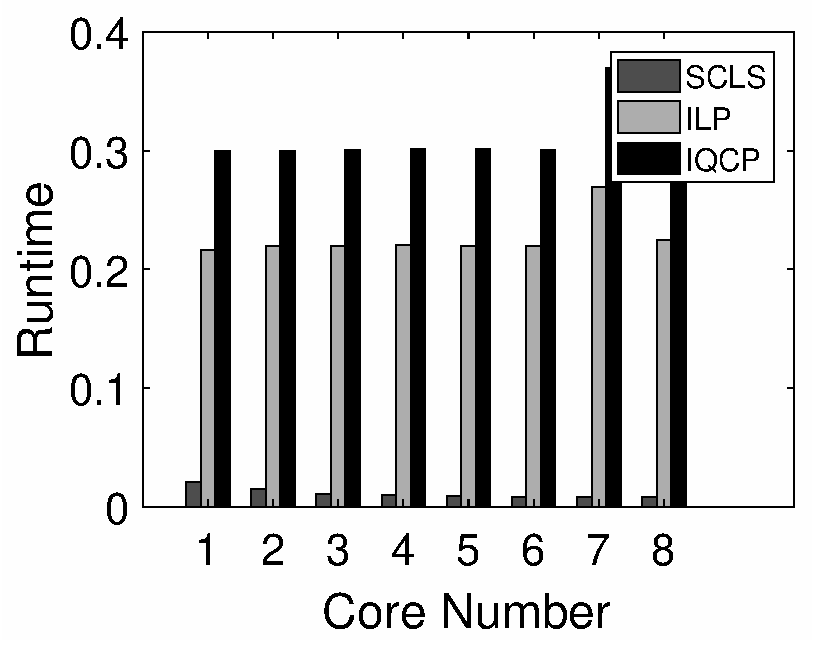
\includegraphics[width=2.25in]{figures/Runtime_noKSP_noCOSE}\\
  \caption{Runtime without CoSE}\label{fig:Runtime_noKSP_noCOSE}
\end{minipage}
\hfill
\begin{minipage}[t]{0.3\linewidth}
\centering
\includegraphics[width=2.25in]{figures/speedup}
\caption{Core speedup}
\label{fig:Speedup}
\end{minipage}
\end{figure*}


\begin{figure*}[tp]
\centering
\begin{minipage}[t]{0.3\linewidth}
\centering
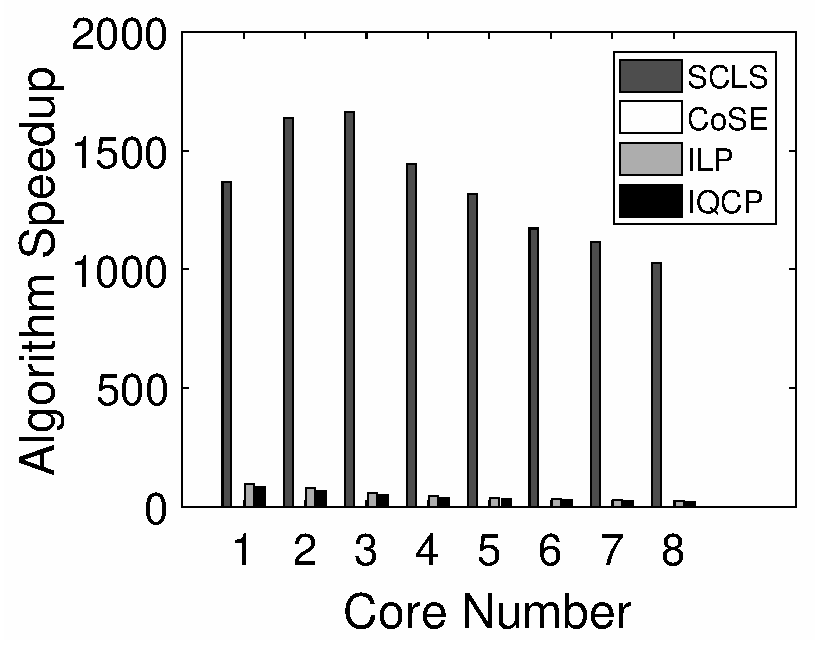
\includegraphics[width=2.25in]{figures/Multiple}
\caption{Algorithm speedup}
\label{fig:Multiple}
\end{minipage}
\hfill
\begin{minipage}[t]{0.3\linewidth}
\centering
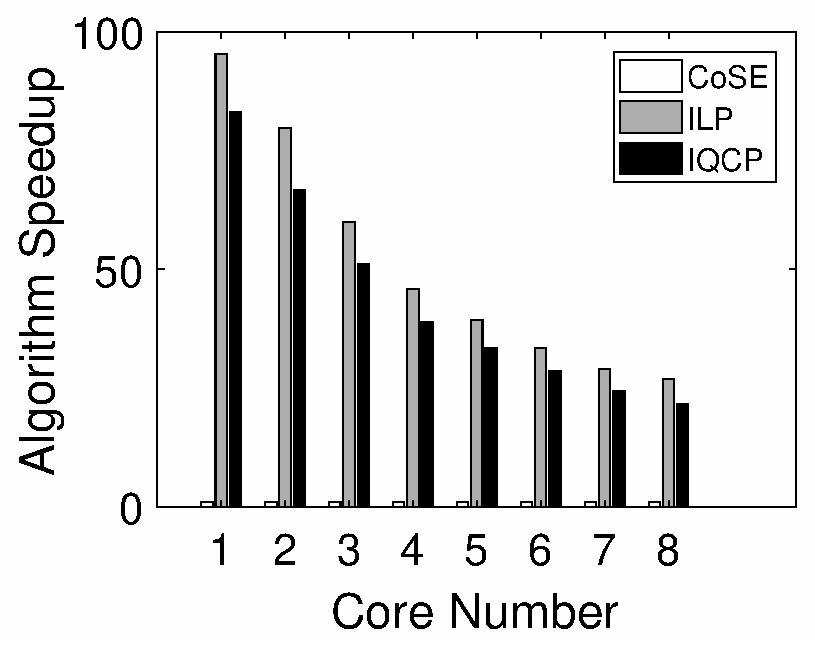
\includegraphics[width=2.25in]{figures/MultipleNoSCLS}
\caption{Algorithm speedup without SCLS}
\label{fig:MultipleNoSCLS}
\end{minipage}
\hfill
\begin{minipage}[t]{0.3\linewidth}
\centering
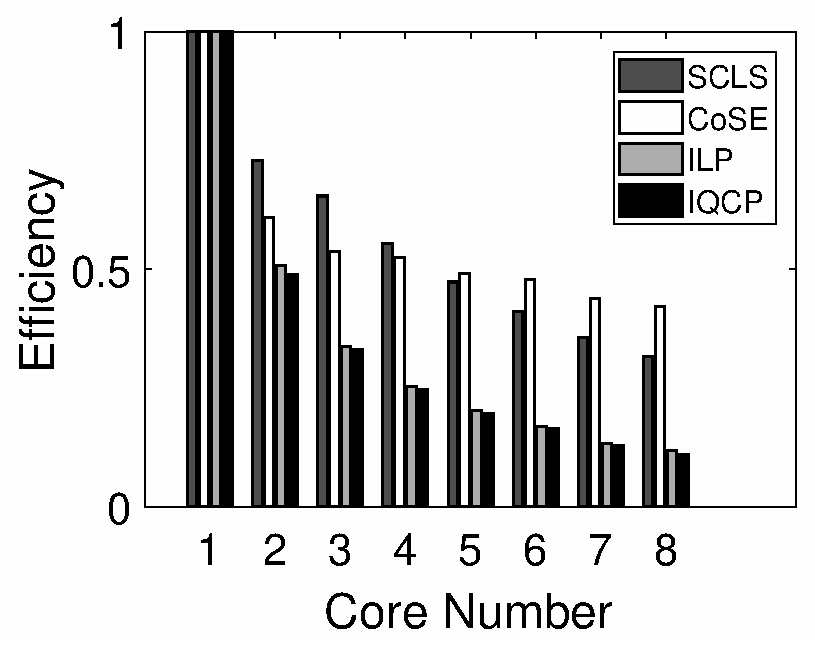
\includegraphics[width=2.25in]{figures/Efficiency}
 \caption{Efficiency}
 \label{fig:Efficiency}
\end{minipage}
\end{figure*}



\subsubsection{Path Hop}
Fig.\ref{fig:normalization hop} shows the path hop of AP, BP, and the sum of both AP and BP. As all algorithms target to minimize the least path weight of the SRLG-disjoint path pair instead of the number of path hops, they have the same AP weight (Fig.\ref{fig:normalization weitgh sum}) even though they have different AP path hops (Fig.\ref{fig:normalization hop}). Although the AP weights under all algorithms are smaller than the BP weights in Fig.\ref{fig:normalization weitgh sum}, in Fig.\ref{fig:normalization hop}, the AP hops may not always be fewer than the BP hops.

%\begin{figure}
%  \centering
%  % Requires \usepackage{graphicx}
%  \includegraphics[width=2.35in]{franz/hop}\\
%  \caption{Path hop}\label{fig:normalization hop}
%\end{figure}

尽管所有算法的AP权重都小于BP权重在图9中,在图10中,AP跳可能并不总是这样比英国石油公司的啤酒花还少。3)运行时:图11显示了不同运行时间下的运行时间算法通过改变CPU核的使用数量。如Cose下的运行时明显大于其他算法,以更清楚地显示其他算法的结果。算法,我们在图12中进一步绘制运行时结果因为ILP和IQCP不是并行算法,的不同数目下的这些算法的运行时。

\subsubsection{Runtime}
\label{subsubsec:Runtime}
Fig.\ref{fig:normalization runtime} shows the run time under different algorithms by varying the number of CPU cores utilized.
As the runtime under CoSE is significantly larger than that under other algorithms, to more clearly show the results of other algorithms, we further plot the runtime results in Fig.\ref{fig:Runtime_noKSP_noCOSE} by excluding CoSE.
As ILP, and IQCP are not parallel algorithms, the runtime of these algorithms under different number of cores is approximately equal. The runtime of our SCLS  and CoSE decreases with the increase of the number of processor cores because these two algorithms can partition the original problem into multiple sub-problems to execute in parallel and take advantage of the parallelism of the multi-core CPU to speed up the path searching process. Although CoSE is a parallel algorithm, the computation time is even larger than  ILP and IQCP. Some possible reasons include 1) the search process to find the conflicting SRLG set in CoSE  is not efficient; 2) As one SRLG usually includes multiple links, the partitioning of problem based on conflicting SRLG will introduce a large number of sub-problems to solve, which also results in a large computation cost.



%\begin{figure}
%  \centering
%  % Requires \usepackage{graphicx}
%  \includegraphics[width=2.35in]{franz/runtime}\\
%  \caption{Runtime}\label{fig:normalization runtime}
%\end{figure}
岩心大致相等。我们的SCLS和COSE随处理器数目的增加而减小。因为这两种算法可以分割原始的问题分成多个子问题并行执行利用多核CPU的并行性加快路径搜索过程。虽然Cose是并行算法,计算时间比ILP和IQCP。一些可能的原因包括:1)搜索在Cose中查找冲突的SRLG集的过程不是2)由于一个SRLG通常包含多个链接,基于冲突SRLG意志的问题划分介绍了大量的子问题需要解决,其中也有一些子问题需要解决。计算量大。与Cose不同的是,我们的SCLS寻找的是一组conf-将AP上的链接切换到陷阱问题中。图中的最小割集理论,实现了图的最短时间。图11。这表明我们的冲突链接集查找算法是有效的,而且我们的分而治之。基于SRLG的智能AP搜索过程及算法冲突链路集可以大大降低计算量。

Different from CoSE, our SCLS looks for the set of conflicting links on an AP caught into the trap problem based on the min-cut theory in graph, and achieves the lowest time in Fig.\ref{fig:normalization runtime}. This demonstrates that our conflicting link set finding algorithm is efficient, and moreover our divide-and-conquer algorithm and intelligent AP searching process based on SRLG Conflicting Link Set can largely reduce the computation cost.

%KSP is known as an effective algorithm to handle the trap problem. However, among all the algorithms implemented, the running time under KSP is the largest. A major problem of KSP is that after the current candidate AP fails the test (that is, it does not have a corresponding disjoint BP), the next candidate AP to be tested is selected solely based on the path length. In the 8 topologies we studied in the trace,  usually a large number of paths need to be tested in order to find a disjoint path pair (if it exists between a pair of nodes), thus KSP needs a large computation time.

\subsubsection{Algorithm speedup}
算法加速:在图14中,我们进一步比较了它们计算速度特别是,找出加速带在使用不同的算法查找所需的路径,我们使用Cose作为基线算法,并设置算法1。=Cose。类似于图11中的结果,SCLS的速度在图14中是Cose的700多倍。类似于图11,因为Cose的运行速度要小得多在图14中很难观察到,我们更进一步将图15中的算法加速比结果排除在最大的一次。

In Fig.\ref{fig:Multiple}, we further compare their computation speeds. Specially, to find out how much speedup is gained when using different algorithms to find the required paths,
%to calculate the algorithm speedup metric,
we use CoSE as the baseline algorithm and set $alg_1$ =CoSE. Similar to the results in the Fig.\ref{fig:normalization runtime}, the speed of SCLS is more than 700 times that of  CoSE in Fig.\ref{fig:Multiple}.  Similar to Fig.\ref{fig:normalization runtime}, as the running speed of CoSE is significantly smaller than others and can hardly be observed in Fig.\ref{fig:Multiple}, we further plot the algorithm speedup results in Fig.\ref{fig:MultipleNoSCLS} by excluding the largest one SCLS.



\subsubsection{Core speedup}

核心加速比:而不是使用算法加速若要比较所有算法的总体运行速度,请将使用公制“核心加速比”来评估数字的核心影响给定的运行速度。算法。图13绘制了所有算法下的核心加速图已执行。算法ILP和IQCP下的核心加速比是在任何核心数下大约等于1,因为它们不是并行算法。我们SCLS的核心加速当核数小于4时,随核心数的增加而增加,在此之后,SCLS的核心加速比保持稳定,即演示4核心对于SCLS来说是足够的。这个结果是符合Amdahl定律[41]的理论核心加速比仅限于由问题确定的上限。尺寸。然而,cose下的运行时继续增加。即使核心数等于8,这是双倍的。数字4。这个结果表明即使是8核cpu。不能满足COSE的并行性要求。这是因为Cose发现的冲突SRLG集包含一个大量的链接,这进一步导致了大量的链接子问题,因此问题的大小和计算量都很大。费用。


Rather than using the algorithm speedup to compare the overall running speeds of all algorithms, the metric "core speedup" is utilized to evaluate how the number of cores in the CPU impacts the running speed of a given algorithm.
Fig.\ref{fig:Speedup} plots the core speedup under all algorithms implemented.
%For the two parallel algorithms SCLS and CoSE, the core speedup   increases with the increase of the number of cores. %\del{Therefore, larger number of cores brings larger performance gain for these two parallel algorithms SCLS and CoSE.}
%However, the increasing speed becomes smaller when the number of cores becomes larger and it incurs a higher cost to coordinate the process.
Core speedup under algorithms ILP and IQCP is  approximately equal to 1 under any core number because they are not parallel algorithms. The core speedup of our SCLS increases with increase of core number when it is less than 4, beyond which the core speedup of SCLS remains stable, which demonstrates that 4 core is sufficient for SCLS. This result is consistent with Amdahl's law\cite{amdahl1967validity} that the theoretical core speedup is limited to a upper bound determined by the problem size. However, the runtime under CoSE continues to increases even though the core number is  equal to 8 which doubles the number 4. This result demonstrates that even 8-core CPU can not satisfy the parallelism requirement in CoSE. This is because the conflicting SRLG set found by CoSE includes  a large number of links,  which further results in a large number of sub-problems  and thus large problem size and  computation cost.


%1) the search
%process to find the conflicting SRLG set in CoSE is not
%efficient; 2) As one SRLG usually includes multiple links,
%the partitioning of problem based on conflicting SRLG will
%introduce a large number of sub-problems to solve, which also
%results in a large computation cost
%
%Among all algorithms, \revtao{the core speedup of our SCLS is the largest except CoSE, which demonstrates that our divide and conquer algorithm designed  based on the SRLG conflicting link set can bring the largest parallelism gain than non-parallel algorithm, and the cardinality of subproblem is smaller than CoSE}.

%\note{How many paths pairs to search in your simulations. If you only search for one pair, then the sub=-problems may be lower than the number of cores, so multi core cannot be used.}
\subsubsection{Efficiency}
%Efficiency is a measure of the overhead due to the parallelization. Programs with a high efficiency spend more time on useful work and less time on synchronization and communications.

效率:类似于图13,涉及更多的核心,效率值随着大量核心数的增加而降低。更多的成本来协调这一过程。在图16中,效率所有算法的值都随着核心号码。与图13中的结果一致,如Cose在核心之后,引入了比我们的scls更多的子问题。数达到4,在Cose下的效率大于。SCLS。然而,我们的SCLS取得了更大的成绩-如图14所示。所有的仿真结果表明,我们的SCLS可以实现。优于其他路由性能更高的方法而在更高的搜索速度,因为冲突找到的链接集可以促进有效的问题划分并行算法执行,计算量小。


Similar to Fig.\ref{fig:Speedup}, with more cores involved, the efficiency value decreases  as a large core number brings more cost to coordinate the process. In Fig.\ref{fig:Efficiency}, the efficiency values of all algorithms decrease with the increase of the core number. Consistent with the results in Fig.\ref{fig:Speedup}, as CoSE introduces more sub-problems than our SCLS, after the core number reaches 4, the efficiency under CoSE is larger than SCLS. However, our SCLS achieves significantly larger algorithm speedup as shown Fig.\ref{fig:Multiple}. %\note{You'd better use the same colore to represent the same algorithm in different figures. It makes reading and understanding difficult with your messy color setup. You may explain what is algorithm speedup and core speedup earlier when you first refer them, although you don't need to give formal definition.}

All the simulation results demonstrate that our SCLS can outperform other approaches with higher routing performance while at a much higher search speed, because the  conflicting link set found can facilitate efficient problem partition for parallel algorithm execution with low computation cost.

